\documentclass[11pt,a4paper]{ctexart}
% Shared preamble for the assignment reports. Use with:
%   \documentclass[11pt,a4paper]{ctexart}  (XeLaTeX)
%   % Shared preamble for the assignment reports. Use with:
%   \documentclass[11pt,a4paper]{ctexart}  (XeLaTeX)
%   % Shared preamble for the assignment reports. Use with:
%   \documentclass[11pt,a4paper]{ctexart}  (XeLaTeX)
%   \input{../common/preamble.tex}
\usepackage[margin=2.3cm]{geometry}
\setmainfont{texgyretermes}[Extension=.otf,UprightFont=*-regular,BoldFont=*-bold,ItalicFont=*-italic,BoldItalicFont=*-bolditalic]
\setsansfont{texgyreheros}[Extension=.otf,UprightFont=*-regular,BoldFont=*-bold,ItalicFont=*-italic,BoldItalicFont=*-bolditalic]
\setmonofont{texgyrecursor}[Extension=.otf,UprightFont=*-regular,BoldFont=*-bold,ItalicFont=*-italic,BoldItalicFont=*-bolditalic]
\usepackage{amsmath,amssymb,mathtools,bm}
\usepackage{graphicx}
\usepackage{booktabs,multirow,makecell,array,tabularx}
\usepackage[table]{xcolor}
\usepackage[most]{tcolorbox}
\usepackage{enumitem}
\usepackage{listings}
\usepackage{subcaption}
\usepackage{siunitx}
\usepackage[hidelinks]{hyperref}
\usepackage[nameinlink,noabbrev]{cleveref}
\usepackage{float}

\setlength{\emergencystretch}{3em}
\linespread{1.15}
\setlist{leftmargin=*,itemsep=2pt,topsep=3pt}
\graphicspath{{figures/}}

\crefname{figure}{图}{图}
\crefname{table}{表}{表}
\crefname{section}{第}{第}
\creflabelformat{section}{#2#1#3 节}
\crefname{equation}{式}{式}
\crefformat{equation}{式~(#2#1#3)}

\lstset{basicstyle=\ttfamily\footnotesize,columns=fullflexible,breaklines=true,frame=single,
  framerule=0.3pt,rulecolor=\color{black!40},backgroundcolor=\color{black!3},
  keywordstyle=\color{blue!60!black}\bfseries,commentstyle=\color{green!40!black},
  numbers=left,numberstyle=\tiny\color{black!50},xleftmargin=1.5em}

% Interview boxes: question, model answer, common wrong answer.
\newtcolorbox{iqbox}[1]{enhanced,breakable,colback=blue!3,colframe=blue!45!black,boxrule=0.5pt,arc=1.5pt,
  left=4pt,right=4pt,top=3pt,bottom=3pt,fonttitle=\bfseries\small,title={面试追问：#1}}
\newtcolorbox{findingbox}[1][]{enhanced,breakable,colback=green!3,colframe=green!40!black,boxrule=0.5pt,arc=1.5pt,
  left=4pt,right=4pt,top=3pt,bottom=3pt,fonttitle=\bfseries\small,title={结论#1}}
\newtcolorbox{caveatbox}{enhanced,breakable,colback=orange!4,colframe=orange!60!black,boxrule=0.5pt,arc=1.5pt,
  left=4pt,right=4pt,top=3pt,bottom=3pt,fonttitle=\bfseries\small,title={不能推出的结论}}

\newcommand{\authorline}{ShaneLiu04\thanks{GitHub: \url{https://github.com/ShaneLiu04}。代码与原始指标见 edge-deploy 仓库各 lab 的 \texttt{artifacts/raw/}。本文基于公开课程材料独立完成，与课程团队无隶属关系。}}

\usepackage[margin=2.3cm]{geometry}
\setmainfont{texgyretermes}[Extension=.otf,UprightFont=*-regular,BoldFont=*-bold,ItalicFont=*-italic,BoldItalicFont=*-bolditalic]
\setsansfont{texgyreheros}[Extension=.otf,UprightFont=*-regular,BoldFont=*-bold,ItalicFont=*-italic,BoldItalicFont=*-bolditalic]
\setmonofont{texgyrecursor}[Extension=.otf,UprightFont=*-regular,BoldFont=*-bold,ItalicFont=*-italic,BoldItalicFont=*-bolditalic]
\usepackage{amsmath,amssymb,mathtools,bm}
\usepackage{graphicx}
\usepackage{booktabs,multirow,makecell,array,tabularx}
\usepackage[table]{xcolor}
\usepackage[most]{tcolorbox}
\usepackage{enumitem}
\usepackage{listings}
\usepackage{subcaption}
\usepackage{siunitx}
\usepackage[hidelinks]{hyperref}
\usepackage[nameinlink,noabbrev]{cleveref}
\usepackage{float}

\setlength{\emergencystretch}{3em}
\linespread{1.15}
\setlist{leftmargin=*,itemsep=2pt,topsep=3pt}
\graphicspath{{figures/}}

\crefname{figure}{图}{图}
\crefname{table}{表}{表}
\crefname{section}{第}{第}
\creflabelformat{section}{#2#1#3 节}
\crefname{equation}{式}{式}
\crefformat{equation}{式~(#2#1#3)}

\lstset{basicstyle=\ttfamily\footnotesize,columns=fullflexible,breaklines=true,frame=single,
  framerule=0.3pt,rulecolor=\color{black!40},backgroundcolor=\color{black!3},
  keywordstyle=\color{blue!60!black}\bfseries,commentstyle=\color{green!40!black},
  numbers=left,numberstyle=\tiny\color{black!50},xleftmargin=1.5em}

% Interview boxes: question, model answer, common wrong answer.
\newtcolorbox{iqbox}[1]{enhanced,breakable,colback=blue!3,colframe=blue!45!black,boxrule=0.5pt,arc=1.5pt,
  left=4pt,right=4pt,top=3pt,bottom=3pt,fonttitle=\bfseries\small,title={面试追问：#1}}
\newtcolorbox{findingbox}[1][]{enhanced,breakable,colback=green!3,colframe=green!40!black,boxrule=0.5pt,arc=1.5pt,
  left=4pt,right=4pt,top=3pt,bottom=3pt,fonttitle=\bfseries\small,title={结论#1}}
\newtcolorbox{caveatbox}{enhanced,breakable,colback=orange!4,colframe=orange!60!black,boxrule=0.5pt,arc=1.5pt,
  left=4pt,right=4pt,top=3pt,bottom=3pt,fonttitle=\bfseries\small,title={不能推出的结论}}

\newcommand{\authorline}{ShaneLiu04\thanks{GitHub: \url{https://github.com/ShaneLiu04}。代码与原始指标见 edge-deploy 仓库各 lab 的 \texttt{artifacts/raw/}。本文基于公开课程材料独立完成，与课程团队无隶属关系。}}

\usepackage[margin=2.3cm]{geometry}
\setmainfont{texgyretermes}[Extension=.otf,UprightFont=*-regular,BoldFont=*-bold,ItalicFont=*-italic,BoldItalicFont=*-bolditalic]
\setsansfont{texgyreheros}[Extension=.otf,UprightFont=*-regular,BoldFont=*-bold,ItalicFont=*-italic,BoldItalicFont=*-bolditalic]
\setmonofont{texgyrecursor}[Extension=.otf,UprightFont=*-regular,BoldFont=*-bold,ItalicFont=*-italic,BoldItalicFont=*-bolditalic]
\usepackage{amsmath,amssymb,mathtools,bm}
\usepackage{graphicx}
\usepackage{booktabs,multirow,makecell,array,tabularx}
\usepackage[table]{xcolor}
\usepackage[most]{tcolorbox}
\usepackage{enumitem}
\usepackage{listings}
\usepackage{subcaption}
\usepackage{siunitx}
\usepackage[hidelinks]{hyperref}
\usepackage[nameinlink,noabbrev]{cleveref}
\usepackage{float}

\setlength{\emergencystretch}{3em}
\linespread{1.15}
\setlist{leftmargin=*,itemsep=2pt,topsep=3pt}
\graphicspath{{figures/}}

\crefname{figure}{图}{图}
\crefname{table}{表}{表}
\crefname{section}{第}{第}
\creflabelformat{section}{#2#1#3 节}
\crefname{equation}{式}{式}
\crefformat{equation}{式~(#2#1#3)}

\lstset{basicstyle=\ttfamily\footnotesize,columns=fullflexible,breaklines=true,frame=single,
  framerule=0.3pt,rulecolor=\color{black!40},backgroundcolor=\color{black!3},
  keywordstyle=\color{blue!60!black}\bfseries,commentstyle=\color{green!40!black},
  numbers=left,numberstyle=\tiny\color{black!50},xleftmargin=1.5em}

% Interview boxes: question, model answer, common wrong answer.
\newtcolorbox{iqbox}[1]{enhanced,breakable,colback=blue!3,colframe=blue!45!black,boxrule=0.5pt,arc=1.5pt,
  left=4pt,right=4pt,top=3pt,bottom=3pt,fonttitle=\bfseries\small,title={面试追问：#1}}
\newtcolorbox{findingbox}[1][]{enhanced,breakable,colback=green!3,colframe=green!40!black,boxrule=0.5pt,arc=1.5pt,
  left=4pt,right=4pt,top=3pt,bottom=3pt,fonttitle=\bfseries\small,title={结论#1}}
\newtcolorbox{caveatbox}{enhanced,breakable,colback=orange!4,colframe=orange!60!black,boxrule=0.5pt,arc=1.5pt,
  left=4pt,right=4pt,top=3pt,bottom=3pt,fonttitle=\bfseries\small,title={不能推出的结论}}

\newcommand{\authorline}{ShaneLiu04\thanks{GitHub: \url{https://github.com/ShaneLiu04}。代码与原始指标见 edge-deploy 仓库各 lab 的 \texttt{artifacts/raw/}。本文基于公开课程材料独立完成，与课程团队无隶属关系。}}


\title{端侧推理内核的跨平台复现报告：\\从 4 核 Ice Lake 虚拟机到 Sapphire Rapids 服务器与 RTX 6000D}
\author{\authorline}
\date{2026 年 11 月}

\begin{document}
\maketitle

\begin{abstract}
edge-deploy 仓库的 edge-runtime 系列 lab（主机屋顶、int8 卷积 / GEMM、卷积算法、DMA 双缓冲、张量程序调优、Q4 GEMV）最初都在一台
4 核 Ice Lake-SP 虚拟机上完成。本报告把同一份代码搬到 AutoDL 上的 2 × Xeon Platinum 8470Q（Sapphire Rapids，AVX-512 + VNNI + AMX-INT8）
和 RTX 6000D（sm\_120，84 GB GDDR7）上重跑，新增 AMX tile GEMM、1--16 线程扫描与 Triton 融合反量化 GEMV，
目的是回答一个面试里常被追问的问题：\emph{一个在开发机上测出来的优化结论，换一台机器还成立吗？}

主要结论：
（a）单核带宽几乎不随“服务器更强”而提高：1 线程 DRAM 读 13.4 → 17.5 GB/s（1.30 倍），16 线程才到 193.5 GB/s；计算峰值随线程数近乎线性，DRAM 在 8 线程后弯曲；
（b）AMX 在 $512^3$ 上 1704 GOP/s，是 VNNI 打包 GEMM 的 3.0 倍，LLM prefill 形状上 5.9 倍，但 $K{=}24$ 的 MobileNetV2 1×1 层被补零到 64 后只有 VNNI 的 0.6 倍；
GEMM 变快后，单独一遍的 requant 从损失 12\% 变成损失 43\%；
（c）有三条结论在新机器上\emph{翻转}：Winograd F(2,3) 在 $56^2$ 层上从快 16\% 变成慢 32\%，512 位向量从“中位数慢 12\%”变成“前 8 名全部更快”，
两线程软件双缓冲在服务器上所有工作量下都慢于串行（0.63--0.95 倍）；编译器也会翻转结论：同一段标量 int8 循环 GCC 13 自动向量化成 VNNI（100 GOP/s），GCC 11 只有 20；
（d）在 GPU 上，融合反量化的 Q4\_0 GEMV 在大矩阵上读到 1327 GB/s（实测带宽的 99.5\%），时间严格按字节缩放；
但 eager 下发有约 22 µs 的地板，只有 CUDA graph 才能把 Q4 的 3.6 倍字节优势兑现成 3.1 倍的解码速度（预测 284 对 92 tok/s）；
（e）CPU 上 Q4 是指令受限的：1、4、16 线程下 Q4 × Q8 与 Q8 × Q8 相差都不到 6\%。
\end{abstract}

\tableofcontents
\newpage

\section{为什么要换机器重跑}

端侧部署的面试题几乎都围绕“瓶颈在哪里”展开：是带宽、算力、下发开销，还是数据布局？一台机器上的测量只能给出一个点，
很多“经验法则”（Winograd 更快、512 位向量会降频、双缓冲能隐藏拷贝、4 bit 权重解码更快）其实是\emph{某个硬件区间}上的结论。
把同一份代码放到参数差别很大的第二台机器上，可以区分两类结论：
\begin{itemize}
  \item \textbf{结构性的}：由算法的访存/计算比决定，换机器只改变常数，例如 depthwise 的 NHWC 布局优势、融合反量化的必要性；
  \item \textbf{位置性的}：取决于两个量的相对大小（GEMM 速度对变换开销、拷贝对计算、K 对 tile 宽度），换机器就可能翻转。
\end{itemize}
本报告的每一节都会标出结论属于哪一类。跨主机的 34 项指标汇总在仓库的 \nolinkurl{interview/CROSS-HOST.md}，由 \nolinkurl{scripts/compare_hosts.py} 生成。

\section{实验平台与方法}

\begin{table}[H]
\centering\small
\caption{三个平台}\label{tab:hosts}
\begin{tabularx}{\linewidth}{>{\raggedright\arraybackslash}p{1.5cm} >{\raggedright\arraybackslash}X >{\raggedright\arraybackslash}X >{\raggedright\arraybackslash}X}
\toprule
 & 本地 VM & 服务器 CPU & 服务器 GPU \\
\midrule
型号 & Xeon Ice Lake-SP（Family 6 Model 106） & 2 × Xeon Platinum 8470Q（Sapphire Rapids） & RTX 6000D（sm\_120） \\
规模 & 4 核 / 8 线程 & 104 核 / 208 线程，每插槽 105 MB L3 & 156 SM，112 MB L2，84 GB GDDR7 \\
ISA / 单元 & AVX-512、VNNI & AVX-512、VNNI、\textbf{AMX-INT8} & Tensor Core（bf16 实测 229 TFLOP/s） \\
内存 & 实测 1 线程 13.4 GB/s & 每插槽 8 × DDR5-4800（理论 307 GB/s） & 实测读 1333 GB/s、拷贝 1280 GB/s \\
编译器 & MinGW GCC 13.2 & GCC 11.4 & CUDA 12.8、Triton \\
\bottomrule
\end{tabularx}
\end{table}

\paragraph{隔离。} 服务器上的 CPU 实验用 \texttt{taskset} 绑在 NUMA1 的物理核（60--75），避开同一插槽上的超线程兄弟核；
GPU 作业通过一个串行队列执行，任何两个 GPU 计时都不重叠。容器的 cgroup 只给 22 个 CPU 的配额，并且宿主上还有其他租户（load average 约 12），
所以 16 线程的个别数字可能被限流；后文只采用单调、可重复的结论，并在每节注明。

\paragraph{计时。} CPU 内核 15 次重复取中位数，每次先扫一遍缓冲区以排除首次缺页；GPU 计时用 CUDA event，
“L2 冷”指轮换足够多份权重拷贝，使总工作集 $\ge 4$ GB（远超 112 MB L2）。

\paragraph{计数器。} 两台机器都没有硬件性能计数器权限（GPU 上 \texttt{ncu} 报 \texttt{ERR\_NVGPUCTRPERM}），
所以“受带宽限制”的判断都来自“墙钟时间 ÷ 字节数”与实测峰值的比较，而不是事务计数。这是本报告最大的方法局限。

\section{主机屋顶：单核带宽与多核扩展}\label{sec:roofline}

\begin{figure}[H]
\centering
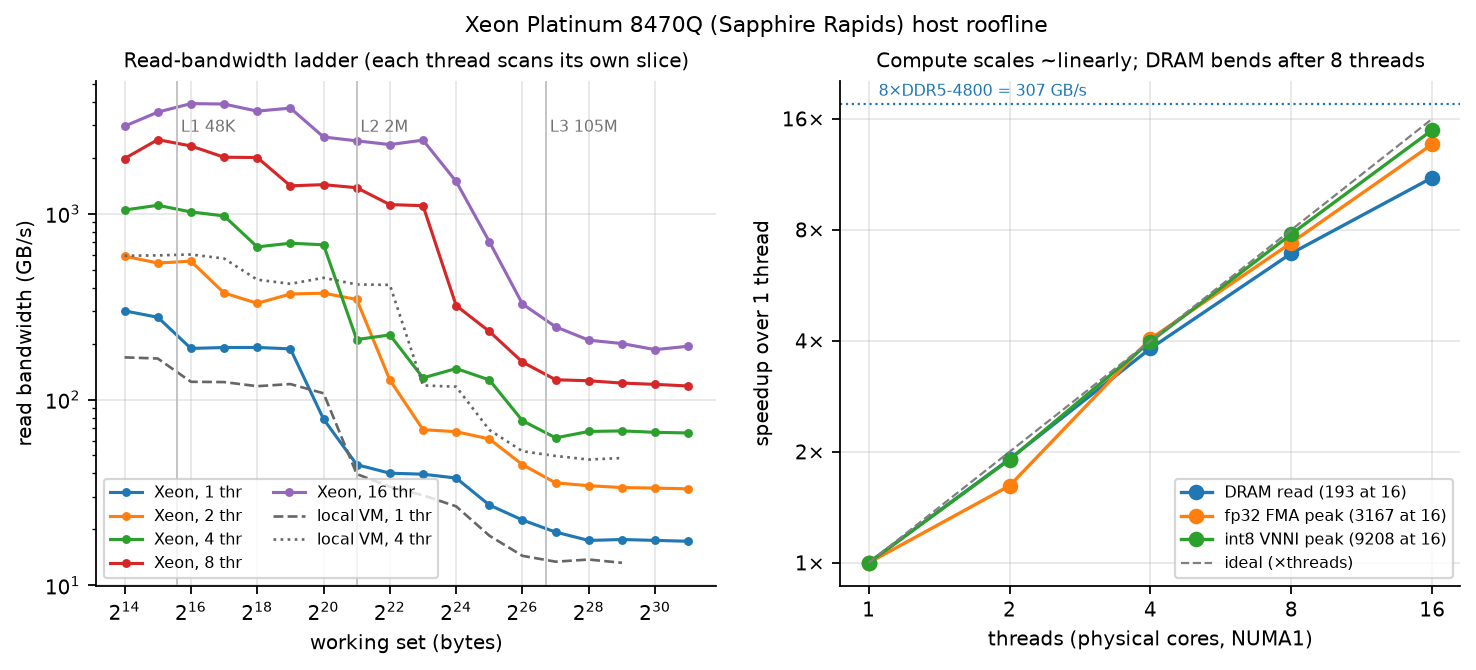
\includegraphics[width=\linewidth]{../../solutions/edge-runtime/host-roofline/artifacts/figures/xeon8470q/thread_scaling.png}
\caption{左：每条线程数的读带宽随工作集变化（灰色虚线为本地 VM）；右：16 线程内的加速比。}\label{fig:scaling}
\end{figure}

\begin{table}[H]
\centering\small
\caption{Xeon 8470Q 屋顶参数随线程数的变化}\label{tab:roof}
\begin{tabular}{rrrrrrr}
\toprule
线程 & L1 读 GB/s & DRAM 读 GB/s & fp32 GFLOP/s & int8 GOP/s & int8/fp32 & fp32 拐点 FLOP/B \\
\midrule
1 & 277 & 17.5 & 232 & 617 & 2.66 & 13.3 \\
2 & 555 & 33.4 & 375 & 1176 & 3.13 & 11.2 \\
4 & 1045 & 66.6 & 939 & 2457 & 2.62 & 14.1 \\
8 & 2311 & 120.6 & 1712 & 4806 & 2.81 & 14.2 \\
16 & 3515 & 193.5 & 3167 & 9208 & 2.91 & 16.4 \\
\bottomrule
\end{tabular}
\end{table}

\begin{findingbox}[：单核带宽是延迟受限的]
1 线程 DRAM 读 17.5 GB/s 只比本地 VM 高 30\%。单核能维持的带宽约等于“在途缺失数 × 64 B ÷ 访存延迟”（Little 定律）；
每核的 line fill buffer 数量在两代之间几乎没变，而 SPR 的 mesh 更大、延迟更长，所以单核带宽几乎原地踏步。
16 线程 193.5 GB/s 是单插槽理论值的 63\%，仍未饱和；8 → 16 线程只涨 1.6 倍，DRAM 曲线在 \cref{fig:scaling} 右图中离开对角线。
\end{findingbox}

计算峰值几乎线性：fp32 从 232 到 3167 GFLOP/s（13.7 倍），int8 从 617 到 9208 GOP/s（14.9 倍）。由 1 线程 fp32 232 GFLOP/s 反推
$232/64 = 3.6$ GHz（单核睿频，两个 512 位 FMA 端口 × 16 lane × 2 FLOP），16 线程每核 198 GFLOP/s 对应 3.1 GHz。
因为计算扩展得比带宽快，拐点（roofline~\cite{roofline} 上算力与带宽相交的强度）随线程数从 13.3 升到 16.4 FLOP/B——\emph{多核让更多的层变成带宽受限}。

\begin{iqbox}{服务器内存带宽有几百 GB/s，为什么单线程解码 7B 模型还是很慢？}
那几百 GB/s 是整个插槽所有内存通道并发时的数字。单线程只能靠自己核里的十几个在途缺失请求去拉数据，按 Little 定律
$B_{\text{core}} \approx N_{\text{inflight}} \times 64\,\text{B} / t_{\text{lat}}$，延迟约 100 ns 时上限就是二十 GB/s 左右；本机实测 17.5 GB/s。
llama.cpp~\cite{llamacpp} 单线程解码 Qwen2.5-7B Q4\_0 实测 3.97 tok/s，乘以每 token 读的 4.1 GB 权重（文件 4.43 GB 减去解码不读的嵌入表）是 16.3 GB/s，单核带宽的 93\%：单线程解码就是在测单核带宽。
\end{iqbox}

\section{int8 GEMM：VNNI、AMX 与 epilogue}\label{sec:int8}

int8-kernels lab 实现了 7 种 int8 GEMM：标量、逐点积 VNNI、按 $[N/16][K/4][16][4]$ 打包 B 的 VNNI、打包 + 寄存器内融合 requant，
以及服务器上新增的 AMX 路径。AMX 用 \texttt{arch\_prctl(ARCH\_REQ\_XCOMP\_PERM, XFEATURE\_XTILEDATA)} 向内核申请 tile 状态，
配置 8 个 16 行 × 64 字节的 tile：tmm0--3 做 2×2 的 int32 累加块，tmm4--5 读 A，tmm6--7 读 VNNI 打包后的 B，
\texttt{\_tile\_dpbusd} 一条指令完成 $16\times16\times64$ 的 u8 × s8 乘加。K 不是 64 的倍数时在打包阶段补零。

\begin{table}[H]
\centering\small
\caption{Xeon 8470Q 单线程 int8 GEMM（GOP/s），全部输出与参考逐位相等}\label{tab:gemm}
\resizebox{\linewidth}{!}{\begin{tabular}{lrrrrrr}
\toprule
形状 & fp32 & 标量 & VNNI 打包 & 打包 + 融合 requant & \textbf{AMX} & AMX + SIMD requant \\
\midrule
pw\_expand\_56（K=24） & 71.2 & 8.5 & 270.2 & 102.3 & 162.4 & 72.3 \\
pw\_expand\_14（K=96） & 85.3 & 19.6 & 476.9 & 268.3 & 693.7 & 296.0 \\
pw\_project\_56（K=144） & 60.4 & 22.3 & 431.7 & 254.5 & 887.6 & 330.8 \\
pw\_head\_7（K=320） & 56.6 & 20.0 & 514.0 & 405.4 & 1208.2 & 701.0 \\
square\_512 & 75.2 & 20.0 & 562.8 & 483.1 & 1703.6 & 968.9 \\
pw\_project\_14（K=576） & 82.3 & 20.2 & 621.7 & 519.3 & 1894.6 & 1140.5 \\
llm\_prefill 256×4096×4096 & 18.4 & 19.9 & 280.1 & 280.3 & 1658.7 & 1453.1 \\
\bottomrule
\end{tabular}}
\end{table}

\begin{figure}[H]
\centering
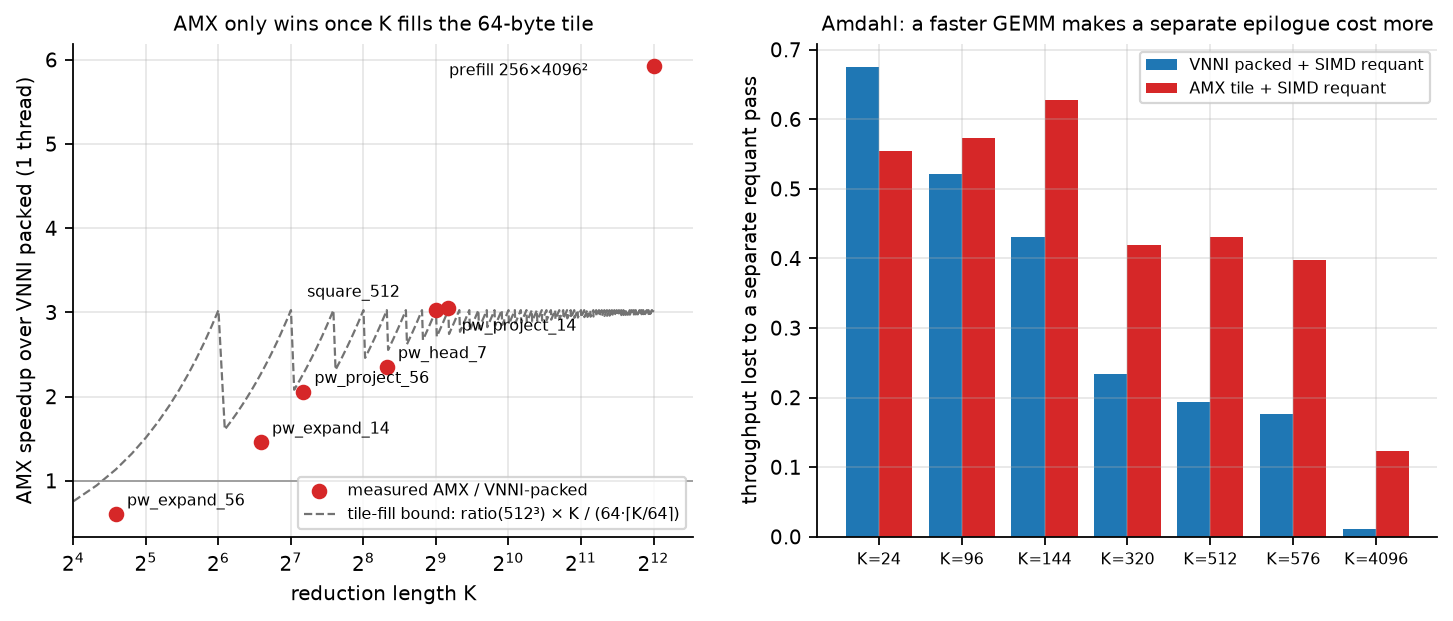
\includegraphics[width=\linewidth]{../../solutions/edge-runtime/int8-kernels/artifacts/figures/xeon8470q/amx_vs_k.png}
\caption{左：AMX 对 VNNI 打包的加速比随 K 变化，虚线为只考虑补零的上界；右：单独一遍 SIMD requant 造成的吞吐损失。}\label{fig:amx}
\end{figure}

\subsection{AMX 的收益正比于 K 的填充率}
一个 AMX tile 在 K 方向一次吃 64 字节。若真实 K 不是 64 的倍数，实际执行的乘加数为 $64\lceil K/64\rceil$，有效比例
\[
  \eta(K) = \frac{K}{64\lceil K/64\rceil}.
\]
把 $512^3$ 上的实测比值 3.03 当作满填充时的比值，上界即 $3.03\,\eta(K)$，这就是 \cref{fig:amx} 左图的锯齿线：
K 刚超过 64 的整数倍时浪费最大，曲线跳水。$K{=}24$ 时 $\eta=0.375$，上界 1.14，实测 0.60——补零之外，打包与 tile 配置的固定成本在这么小的 K 上也摊不开。
MobileNetV2 这类端侧模型的瓶颈层恰好通道很少，所以\emph{AMX 路径必须按层选择，小 K 的层回退到 VNNI}。这是一个典型的“位置性”结论。

\subsection{prefill 形状为什么快 5.9 倍}
prefill 点远高于上界，说明那里的差距不是 tile 填充问题。打包 VNNI 内核的外层循环每处理 4 行 A，就把整个 B（$4096\times4096$ = 16 MiB，远超 2 MiB 的 L2）
从 L3 扫一遍，共 $256/4=64$ 遍；AMX 内核每 32 行（2 个 16 行 tile）扫一遍，只有 8 遍。两者都没有 K/N 方向的 cache 分块，
所以 VNNI 在这个形状上掉到 280 GOP/s，只有 $512^3$ 时的一半；AMX 少流 8 倍的 B，于是快 5.9 倍。
这说明 AMX 的一部分“加速”其实来自更大的寄存器块带来的数据复用，而这本可以通过给 VNNI 内核加 cache 分块拿到——这正是 oneDNN 这类库做的事。

\subsection{峰值利用率}
按每核每周期 2048 次 int8 运算、2.1 GHz 基频估算，单核 AMX 峰值约 4.3 TOP/s；$512^3$ 的 1.7 TOP/s 和 K=576 的 1.9 TOP/s 只是峰值的 40--44\%。
2×2 的输出块里每个 A tile、B tile 只复用 2 次，tile load 的时间没被完全藏住；更大的块受限于只有 8 个 tile 寄存器。

\subsection{Amdahl：GEMM 越快，epilogue 越贵}
\Cref{fig:amx} 右图是“GEMM 之后再单独扫一遍 int32 累加器做 requant”造成的损失。VNNI 列随 K 增大而下降（GEMM 变重，requant 被摊薄）；
AMX 列在 K = 144--576 时稳定在 40\% 左右：requant 的时间不变，GEMM 却快了 3 倍。$512^3$ 上 AMX 从 1704 掉到 969（$-43\%$），
本地 VNNI 只损失 12\%（212 → 186）。若 requant 占比为 $f$，GEMM 加速 $s$ 倍后整体加速只有 $1/((1-f)/s + f)$——要保住 AMX 的收益，
requant 必须融合进 tile store 之后的寄存器阶段。

\subsection{编译器也是一个变量}
同一段标量 int8 点积，本地 GCC 13.2 跑到 100 GOP/s，服务器 GCC 11.4 只有 20 GOP/s——这是 CROSS-HOST 表里唯一一项服务器慢 5 倍的指标。
对两份汇编计数：GCC 13 生成 78 条 \texttt{vpdpbusd}、14 条 \texttt{vpmov[sz]xbw}，GCC 11 只有 60 条 \texttt{vpdpbusd}、80 条字节扩展指令。
GCC 13 把 \texttt{int32 += u8 * s8} 的循环识别成了 VNNI 点积模式，GCC 11 只能先把字节扩成 16 位再乘。
\emph{“标量参考实现”的速度取决于编译器版本}，比较手写内核与参考实现的加速比时，必须同时报告编译器。

\begin{iqbox}{有了 AMX，为什么 oneDNN 仍然保留 VNNI 路径？}
因为 AMX 的收益依赖形状。tile 在 K 方向固定 64 字节、M 方向 16 行：小 K（MobileNet 的 1×1 层 K=24）补零浪费过半，小 M（batch 1 的 GEMV，M=1）浪费 15/16。
实测 K=24 时 AMX 只有 VNNI 的 0.6 倍。另外 AMX 需要进程申请 XTILEDATA 状态、上下文切换要多保存 8 KB 的 tile 寄存器，
对小算子这些固定成本也不可忽略。所以库按形状选路径：大 GEMM（prefill、大 batch）走 AMX，decode 的 GEMV 和小通道卷积走 VNNI / AVX-512。
\end{iqbox}

\section{卷积：Winograd 的收益取决于 GEMM 有多快}\label{sec:conv}

\begin{table}[H]
\centering\small
\caption{ResNet 3×3 卷积单线程 GFLOP/s（Winograd 按直接卷积 FLOP 计等效值）}\label{tab:conv}
\resizebox{\linewidth}{!}{\begin{tabular}{lrrr}
\toprule
层 & implicit GEMM 本地 → 服务器 & Winograd F(2,3) 本地 → 服务器 & Winograd / implicit（服务器） \\
\midrule
3×3，$56^2$，64→64 & 34.3 → 80.4 & 39.7 → 54.3 & \textbf{0.68} \\
3×3，$14^2$，256→256 & 34.9 → 48.2 & 75.0 → 144.5 & 3.00 \\
\bottomrule
\end{tabular}}
\end{table}

Winograd F(2,3)~\cite{lavin2016} 把每个输出 tile 的乘法减少到 $16/36$（2.25 倍），代价是输入、输出两次变换。变换是逐 tile 的加减与散布写，
受访存与标量开销限制，从本地到服务器只快 1.4 倍；而 implicit GEMM 在服务器上快了 2.3 倍（更大的 L2、两个 512 位 FMA 端口）。
设 GEMM 部分的时间为 $t_g$、变换时间为 $t_x$，Winograd 的收益是 $t_g / (t_g/2.25 + t_x)$：当 GEMM 变快、$t_x$ 不变时收益缩小，直至小于 1。
$56^2$ 层通道只有 64，变换的比重高，于是翻转；$14^2$ 层 $K = C\times9 = 2304$ 较大但空间小，GEMM 效率本身偏低，减少乘法仍然划算（3.0 倍，超过理论的 2.25；
一个可能的解释是变换后的 16 个批量 GEMM 形状更规整、比 $14^2$ 的 implicit GEMM 更容易向量化，本仓库没有拆分验证）。depthwise 的布局结论则是结构性的：NHWC + SIMD 比 CHW 快 8.2 倍（本地 9.0 倍）。

\begin{iqbox}{Winograd 一定比 im2col / implicit GEMM 快吗？}
不一定。它用更少的乘法换来变换开销和更差的数值（fp16 下 F(4,3) 的误差是直接卷积的 7.2 倍）。当 GEMM 已经很快（大核、AMX、Tensor Core）、
或者通道数少到变换占比高时，变换成本占主导。本仓库实测：同一层在 Ice Lake 上 Winograd 快 16\%，在 Sapphire Rapids 上慢 32\%。
所以推理框架（如 ARM Compute Library、cuDNN）在运行时按层、按设备测量后选择算法，而不是写死。
\end{iqbox}

\section{DMA 双缓冲：CPU 上的软件流水为何失效}\label{sec:dma}

dma-double-buffer lab 先用闭式模型和事件模拟分析 MCU / PULP（Dory~\cite{dory}）上的 tile 级双缓冲，再在 CPU 上用“一个线程拷贝、一个线程计算”实测。
模型的加速比为
\[
  S = \frac{n(t_c + t_m)}{t_m + (n-1)\max(t_c,t_m) + t_c},
\]
在 $t_c/t_m \approx 1$ 时最大（接近 2）。

\begin{table}[H]
\centering\small
\caption{64 KiB tile，双缓冲对串行的加速比}\label{tab:dma}
\begin{tabular}{lrrrrrrrrr}
\toprule
每字节计算量 & 0 & 1 & 2 & 3 & 4 & 6 & 8 & 16 & 32 \\
\midrule
模型预测（服务器 $c/m$） & 1.00 & 1.53 & 1.94 & 1.71 & 1.62 & 1.36 & 1.24 & 1.13 & 1.08 \\
服务器实测 & 0.83 & 0.63 & 0.72 & 0.75 & 0.70 & 0.78 & 0.76 & 0.93 & 0.95 \\
本地实测 & 0.66 & 0.81 & 1.00 & 1.13 & 1.08 & 1.23 & 1.10 & 1.07 & 1.04 \\
\bottomrule
\end{tabular}
\end{table}

\begin{figure}[H]
\centering
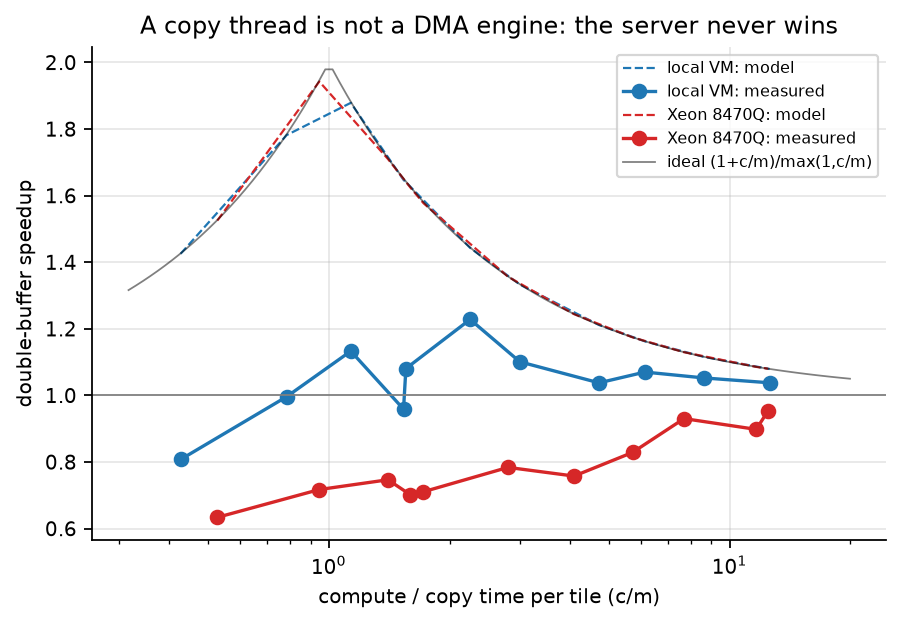
\includegraphics[width=0.8\linewidth]{../../solutions/edge-runtime/dma-double-buffer/artifacts/figures/xeon8470q/model_vs_measured.png}
\caption{模型预测与两台主机的实测。}\label{fig:dma}
\end{figure}

服务器上没有一个点超过 1。更关键的是\emph{形状}：如果损失来自“重叠得不完全”，实测曲线应与模型同形、只是更矮；
实际上服务器曲线整体平移到 1 以下，模型在 $c/m\approx1$ 处的峰完全消失。这说明第二个线程本身带来了固定成本：
双缓冲模型假设拷贝与计算使用互不干扰的资源，而 CPU 上二者都是 load/store、共享 L2/L3 与内存控制器；
服务器上两个线程还可能落在 mesh 上相距较远的核上，每个 tile 交接时所有 cache line 都要跨 mesh 迁移一次。

\begin{iqbox}{为什么双缓冲在 MCU / GPU 上有效，在 CPU 上常常没用？}
双缓冲的前提是“搬运”由独立硬件完成：MCU 的 DMA 控制器、GPU 的 copy engine 与 Hopper 的 TMA，搬运不占计算单元的发射槽，也不污染计算单元的缓存。
CPU 上用另一个线程做 memcpy，搬运与计算争用同一套 load/store 端口和缓存层次，还要付线程同步和 cache line 跨核迁移的成本。
CPU 上真正等价的做法是硬件预取或软件 \texttt{prefetch} 指令，而不是拷贝线程。本仓库实测服务器上 0.63--0.95 倍。
\end{iqbox}

\section{张量程序调优：最优调度不可迁移}\label{sec:tuning}

tensor-program-tuning lab 用 Python 生成 C++ 内核（七个旋钮：外层/内层循环顺序、三维 tile、展开、向量宽度），比较 grid、random、
岭回归代价模型引导、进化四种搜索。服务器上重跑全部 4 种搜索 × 3 个种子：

\begin{table}[H]
\centering\small
\caption{同一搜索空间在两台机器上的结果（GFLOP/s，单线程）}\label{tab:tune}
\resizebox{\linewidth}{!}{\begin{tabular}{lrrrrr}
\toprule
问题 & 最优 本地 → 服务器 & NumPy 1 线程 & 代价模型 Spearman & 前 8 名 256 位 & 前 8 名 512 位 \\
\midrule
square\_256 & 85.7 → 114.7 & 90.1 → 160.6 & 0.47 → 0.54 & 115.1 & \textbf{173.1} \\
pw\_expand\_14 & 84.5 → 112.4 & 95.4 → 166.1 & 0.53 → 0.56 & 111.1 & \textbf{156.5} \\
\bottomrule
\end{tabular}}
\end{table}

两个“位置性”结论：
\begin{itemize}
  \item \textbf{向量宽度翻转}。本地 Ice Lake 上 512 位只有 1/8 的调度更快、中位数慢 12\%；服务器上前 8 名全部更快，最优 173 对 115。
        SPR 的 AVX-512 降频档位更温和，且有两个完整的 512 位 FMA 端口。\texttt{-mprefer-vector-width=512} 本身就是一个需要按目标机器搜索的旋钮。
  \item \textbf{最优调度换位置}。本地前 8 名多是 \texttt{ikji}/\texttt{ijki} 内层、64 宽的 tile；服务器前 8 名有 7 个是 \texttt{iikj} 内层、32×8 tile。
        这就是 AutoTVM~\cite{autotvm} / Ansor~\cite{ansor} 必须在目标设备上测量、并为每种硬件分别保存调优日志的原因。
\end{itemize}
搜索器最优仍低于 NumPy/OpenBLAS（115 对 161）：模板里没有 B 的打包和 K 方向的寄存器分块，搜索只能在给定空间内找最优，空间本身决定上限。

\section{Q4 GEMV：CPU 指令受限，GPU 带宽受限}\label{sec:gemv}

\subsection{CPU：Q4 的字节优势被解包吃掉}

Q4\_0 / Q8\_0 的块布局与 ggml~\cite{llamacpp} 逐字节一致；GPU 侧的融合反量化内核用 Triton~\cite{triton} 编写。

\begin{table}[H]
\centering\small
\caption{Xeon 8470Q，Llama-7B MLP 形状 11008×4096（µs）}\label{tab:gemvcpu}
\begin{tabular}{lrrrr}
\toprule
方法 & 1 线程 & 4 线程 & 16 线程 & 16 线程 GB/s \\
\midrule
fp32 & 9580 & 2545 & 660 & 273 \\
fp16 & 4978 & 1035 & 297 & 304 \\
Q8\_0 浮点融合 & 2400 & 648 & 198 & 242 \\
Q4\_0 先反量化 & 7315 & 1852 & 523 & 48 \\
Q4\_0 浮点融合 & 3545 & 903 & 281 & 90 \\
Q8\_0 × Q8 VNNI & 1947 & 525 & 154 & 311 \\
Q4\_0 × Q8 VNNI & 2057 & 523 & 158 & 161 \\
\bottomrule
\end{tabular}
\end{table}

1、4、16 线程下 Q4 × Q8 与 Q8 × Q8 都相差不到 6\%：Q4 只读一半字节，却没有更快。每 32 个权重 Q4 要多做一次半字节拆分（与、移位）和一次减 8，
这些指令与点积争用同一组向量端口，于是内核是指令受限的。fp32 的 273 GB/s 超过 16 线程 DRAM 只读的 193 GB/s，
说明 180 MB 的权重里仍有一部分留在 105 MB 的 L3 中——单层重复调用的 GEMV 测不出整模型解码。llama.cpp 端到端的结果（单线程 Q4\_0 读到 16.3 GB/s，单核带宽的 93\%）
见 llama-cpp-7b 报告。

\subsection{GPU：融合之后只剩搬字节}

\begin{figure}[H]
\centering
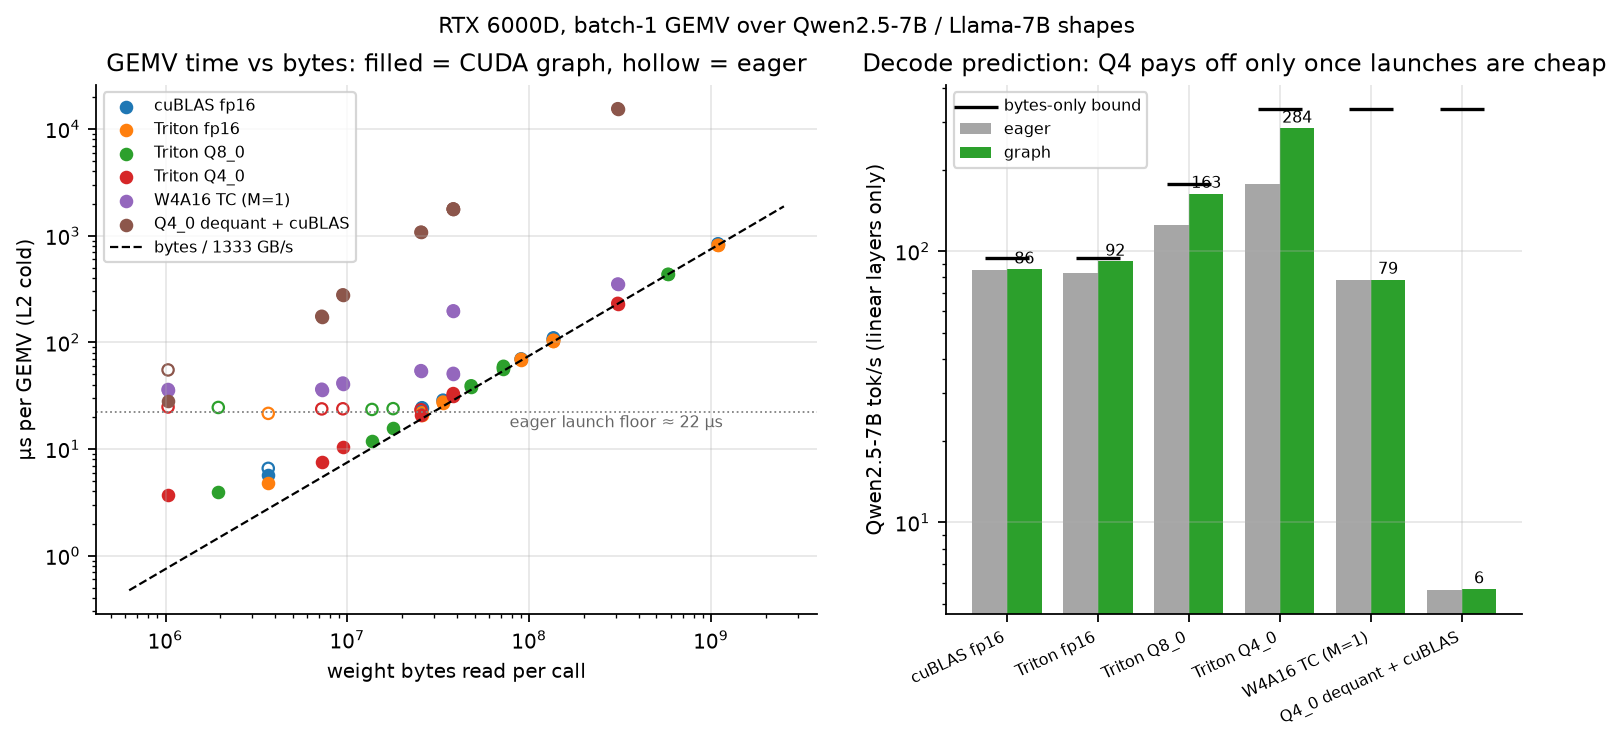
\includegraphics[width=\linewidth]{../../solutions/edge-runtime/q4-gemv/artifacts/figures/gemv_gpu_roofline.png}
\caption{左：每次 GEMV 的时间对读取字节数（实心 = CUDA graph，空心 = eager），虚线为 bytes / 1333 GB/s；右：只算 Linear 的 Qwen2.5-7B 解码预测。}\label{fig:gemvgpu}
\end{figure}

\texttt{gpu/triton\_gemv.py} 把 Q4\_0 的 AoS 块（\texttt{[d fp16][qs]}）转成 SoA，使量化字节与 scale 各自合并访存，
每个 program 处理 \texttt{BN} 行 × \texttt{NB} 个 32 元素块，在寄存器里拆半字节、乘 scale。\Cref{fig:gemvgpu} 左图给出三个区域：
\begin{itemize}
  \item \textbf{30 MB 以上}：所有融合方法的实心点落在 bytes / 1333 GB/s 的虚线上，与格式无关。lm\_head（152064×3584）上 fp16 1344、Q8 1337、Q4 1327 GB/s，
        时间比 838 / 231 = 3.63，恰好是 16 bit 对 4.5 bit 的字节比 3.56。GPU 有足够的 ALU 隐藏解包——与 CPU 正好相反。
  \item \textbf{10 MB 以下}：eager 的空心点贴着约 22 µs 的水平线，这是 Python + Triton 的下发开销，与形状无关（k/v 投影只有 1.8 MB 也要 24.8 µs）；
        CUDA graph 后降到 3.7 µs。Q4 把字节压到 1/3.6，却把更多层推到了这条线下面。
  \item \textbf{不融合}：先反量化成 fp16 再调 cuBLAS（棕色），每次都把 fp16 权重写出再读回，比 fp16 GEMV 还慢 15--70 倍。
\end{itemize}

\begin{table}[H]
\centering\small
\caption{Qwen2.5-7B 解码预测（只算 28 层 Linear + lm\_head）}\label{tab:decode}
\begin{tabular}{lrrrr}
\toprule
方法 & 权重 GB & eager tok/s & graph tok/s & graph 占字节上界 \\
\midrule
cuBLAS fp16 & 14.14 & 85.1 & 85.8 & 91\% \\
Triton fp16 & 14.14 & 83.3 & 91.7 & 97\% \\
Triton Q8\_0 & 7.51 & 124.9 & 163.0 & 92\% \\
Triton Q4\_0 & 3.98 & 176.4 & \textbf{283.7} & 85\% \\
W4A16 Tensor Core（M=1） & 3.98 & 78.1 & 78.6 & 23\% \\
Q4\_0 反量化 + cuBLAS & 3.98 & 5.6 & 5.7 & 2\% \\
\bottomrule
\end{tabular}
\end{table}

Q4 的收益只在 graph 模式下兑现：eager 时 196 个小层每层都吃 22 µs 的地板，Q4 只比 fp16 快 2.1 倍；graph 后 3.1 倍。
W4A16 Tensor Core 内核（\texttt{tl.dot}）在 M=1 时只有上界的 23\%：MMA 的 16 行 tile 有 15 行是空的。

\begin{table}[H]
\centering\small
\caption{batch 扫描，11008×4096（µs）}\label{tab:batch}
\begin{tabular}{rrrr}
\toprule
M & cuBLAS fp16 & W4A16 TC & Q4 反量化 + cuBLAS \\
\midrule
1 & 69.5 & 53.9 & 1077 \\
16 & 72.1 & 67.4 & 1088 \\
32 & 76.4 & 99.9 & 1093 \\
128 & 111.2 & 219.2 & 1108 \\
1024 & 693.4 & 1450.1 & 1416 \\
4096 & 2645.5 & 5630.6 & 3083 \\
\bottomrule
\end{tabular}
\end{table}

$M \le 16$ 时读权重主导，4 bit 权重占优；$M \ge 32$ 进入算力区，我们的 W4A16 内核只有约 65 TFLOP/s（cuBLAS 135），内层循环里的反量化开销显形；
$M\ge1024$ 时连“先反量化再 cuBLAS”都比它快——反量化一次的成本被 1024 行摊薄了。这正是 vLLM 这类引擎在 decode 用 Marlin 类 W4A16、
在 prefill 先反量化或直接用 fp16/fp8 GEMM 的原因。

\begin{iqbox}{4 bit 量化一定让解码变快吗？}
只在“读权重”是瓶颈时成立。三种情况下它不成立：（1）CPU 上解包指令与点积争用向量端口，本仓库 Q4 × Q8 与 Q8 × Q8 一样快；
（2）GPU 上若用 eager 逐层下发，小层被约 22 µs 的固定开销主导，字节省下来也没用；（3）batch 大了进入算力区，反量化变成内层循环的额外指令。
要兑现收益需要：反量化融合进 GEMV、用 CUDA graph 或 persistent kernel 消除下发开销、decode 与 prefill 用不同内核。
\end{iqbox}

\section{跨主机总览}

\begin{figure}[H]
\centering
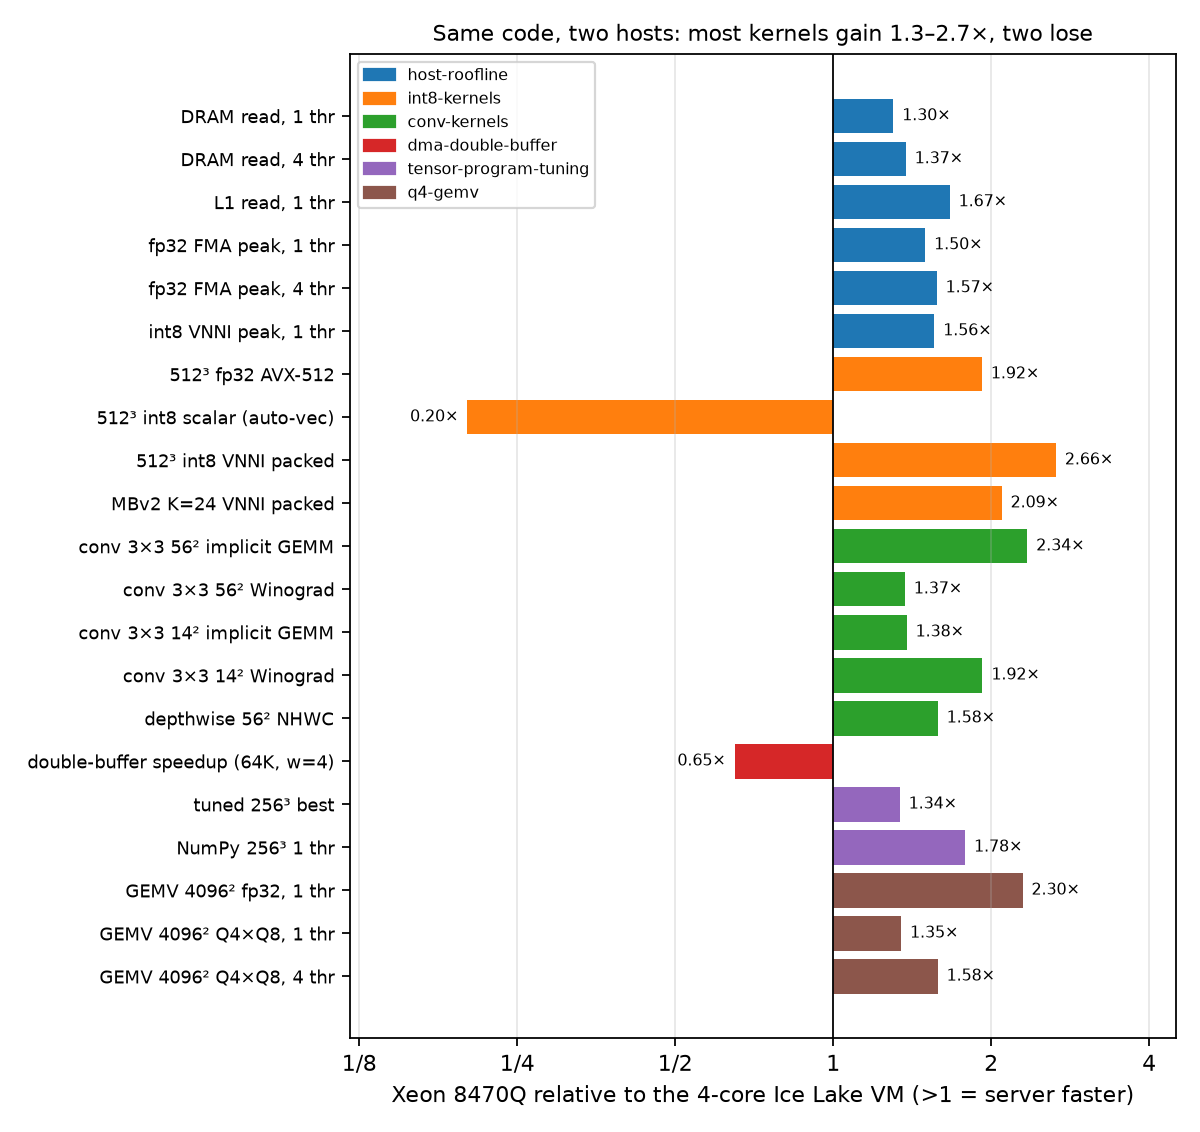
\includegraphics[width=0.92\linewidth]{../../interview/figures/cross_host.png}
\caption{同一代码在两台主机上的比值（µs 类指标已取倒数，大于 1 表示服务器更快）。}\label{fig:cross}
\end{figure}

\Cref{fig:cross} 汇总了 21 项指标。大多数在 1.3--2.7 倍之间，与“单核睿频 + 更大缓存”的量级吻合；两项低于 1：
GCC 11 下的标量 int8（\cref{sec:int8}）与两线程双缓冲（\cref{sec:dma}）。最大的增益（2.3--2.7 倍）出现在 VNNI 打包 GEMM 和 implicit GEMM 卷积上，
它们的工作集受益于 2 MiB L2（Ice Lake VM 为 1.25 MiB）。需要强调：这张图里的“慢”和“快”都不只来自硬件——编译器版本、cgroup 限流、
NUMA 绑定方式都在其中，这也是为什么每个比值都应该能追溯到原始的 \texttt{summary.json}。

\section{面试速答}

\begin{iqbox}{如何判断一个算子是带宽受限还是算力受限？}
算它的算术强度 $I$ = FLOP / 字节，与机器拐点 $P_{\text{peak}}/B$ 比较。本机 1 线程拐点 13.3 FLOP/B、16 线程 16.4 FLOP/B；
GEMV 的强度约 2 FLOP/B（fp16 权重）或 7 FLOP/B（Q4），永远在拐点左边；$512^3$ GEMM 的强度上百，在右边。
注意拐点随线程数、数据类型（int8 峰值是 fp32 的 2.7--3.1 倍）变化，不是常数。没有计数器时，用“实测时间 × 峰值带宽 ÷ 字节数”估计带宽占比。
\end{iqbox}

\begin{iqbox}{CUDA graph 为什么能让小模型 / 小层的解码明显变快？}
eager 模式下每个 kernel 都要经过 Python、框架调度、驱动提交，本机 Triton 约 22 µs 一次，与 kernel 大小无关。
7B 模型每 token 196 次 Linear 调用，光下发就是 4.3 ms，而 Q4 权重全部读完只要 3 ms。CUDA graph 把整串 kernel 一次提交，
每个节点的开销降到几 µs（本机 3.7 µs），使小层回到带宽受限。代价是形状必须固定（静态 KV cache、固定 batch）。
\end{iqbox}

\begin{iqbox}{为什么 GPU 计时要做“L2 冷”？}
RTX 6000D 有 112 MB L2。4096×4096 的 fp16 权重只有 33.5 MB，同一份权重反复调用时会常驻 L2，测出 3975 GB/s——这是 L2 带宽，
而 7B 模型每 token 要读 4--14 GB，必然来自 DRAM。所以要轮换足够多份权重拷贝（总量 $\ge$ 4 GB），每次调用都读冷数据。CPU 上同理：105 MB L3 会让单层 GEMV 测出超过 DRAM 的带宽（\cref{tab:gemvcpu} 的 273 GB/s）。
\end{iqbox}

\begin{caveatbox}
\begin{itemize}
  \item 没有硬件计数器：所有“带宽受限 / 指令受限”的判断来自墙钟时间与实测峰值的比较，没有 DRAM 事务数或端口占用率佐证。
  \item 服务器 cgroup 只给 22 个 CPU 配额且有其他租户；16 线程的个别点（例如 triad 低于只读）可能是被限流的结果，本报告没有用它们下结论。
  \item 两台机器的编译器不同（GCC 13.2 对 11.4），跨主机比值混合了硬件与编译器两个因素；只有标量 int8 一项做了汇编级拆分。
  \item GPU 解码预测只把单层 GEMV 时间相加，没有 attention、归一化、RoPE、采样与层间融合；真实端到端数字见 llama-cpp-7b 报告。
  \item AMX 峰值 4.3 TOP/s 是按规格估算的，利用率 40--44\% 受这个估算影响。
\end{itemize}
\end{caveatbox}

\section{复现}

\begin{lstlisting}[language=bash,numbers=none]
# 服务器 CPU：结果写入各 lab 的 artifacts/raw/，入库时放到 artifacts/raw/xeon8470q/
cd solutions/edge-runtime/host-roofline
EDGE_THREADS=1,2,4,8,16 taskset -c 60-75 python scripts/run_experiments.py --max-mib 2048
cd ../int8-kernels && taskset -c 60 python scripts/run_experiments.py --only gemm
# GPU
cd ../q4-gemv && python gpu/bench_gpu.py check && python gpu/bench_gpu.py all
# 汇总与作图（本地即可）
python scripts/compare_hosts.py && python scripts/plot_server.py
\end{lstlisting}

\begin{thebibliography}{99}
\bibitem{roofline} S. Williams, A. Waterman, D. Patterson. Roofline: An Insightful Visual Performance Model for Multicore Architectures. \emph{Communications of the ACM}, 52(4), 2009.
\bibitem{lavin2016} A. Lavin, S. Gray. Fast Algorithms for Convolutional Neural Networks. In \emph{CVPR}, 2016.
\bibitem{dory} A. Burrello, A. Garofalo, N. Bruschi, G. Tagliavini, D. Rossi, F. Conti. DORY: Automatic End-to-End Deployment of Real-World DNNs on Low-Cost IoT MCUs. \emph{IEEE Transactions on Computers}, 70(8), 2021.
\bibitem{autotvm} T. Chen, L. Zheng, E. Yan, Z. Jiang, T. Moreau, L. Ceze, C. Guestrin, A. Krishnamurthy. Learning to Optimize Tensor Programs. In \emph{NeurIPS}, 2018.
\bibitem{ansor} L. Zheng, C. Jia, M. Sun, Z. Wu, C. H. Yu, A. Haj-Ali, Y. Wang, J. Yang, D. Zhuo, K. Sen, J. E. Gonzalez, I. Stoica. Ansor: Generating High-Performance Tensor Programs for Deep Learning. In \emph{OSDI}, 2020.
\bibitem{llamacpp} G. Gerganov et al. llama.cpp / ggml. \url{https://github.com/ggml-org/llama.cpp}, 2026.
\bibitem{triton} P. Tillet, H. T. Kung, D. Cox. Triton: An Intermediate Language and Compiler for Tiled Neural Network Computations. In \emph{MAPL}, 2019.
\end{thebibliography}

\end{document}
